%=============================================================================
%=============================================================================

\chapter{Introduction}
\label{ch-Introduction}

This manual describes \hypre{}, a software library of high performance
preconditioners and solvers for the solution of large, sparse linear systems of
equations on massively parallel computers \cite{RDFalgout_JEJones_UMYang_2004TA}.  The \hypre{} library was created
with the primary goal of providing users with advanced parallel preconditioners.
The library features parallel multigrid solvers for both structured and
unstructured grid problems.  For ease of use, these solvers are accessed from
the application code via \hypre{}'s conceptual linear system interfaces \cite{RDFalgout_JEJones_UMYang_2005a}
(abbreviated to {\em conceptual interfaces} throughout much of this manual),
which allow a variety of natural problem descriptions.

This introductory chapter provides an overview of the various features in
\hypre{}, discusses further sources of information on \hypre{}, and
offers suggestions on how to get started.

%-----------------------------------------------------------------------------

\section{Overview of Features}
\label{Features}

\begin{itemize}

\item
{\bf Scalable preconditioners provide efficient solution on today's
and tomorrow's systems:} \hypre{} contains several families of
preconditioner algorithms focused on the scalable solution of {\it
very large} sparse linear systems. (Note that small linear systems,
systems that are solvable on a sequential computer, and dense systems
are all better addressed by other libraries that are designed
specifically for them.)
\hypre{} includes ``grey-box'' algorithms
that use more than just the matrix to solve certain classes of
problems more efficiently than general-purpose libraries. This
includes algorithms such as structured multigrid.


\item
{\bf Suite of common iterative methods provides options for a spectrum
of problems:} \hypre{} provides several of the most commonly used
Krylov-based iterative methods to be used in conjunction with its
scalable preconditioners. This includes methods for nonsymmetric
systems such as GMRES and methods for symmetric matrices such as
Conjugate Gradient.

\item
{\bf Intuitive grid-centric interfaces obviate need for complicated
data structures and provide access to advanced solvers:} \hypre{} has
made a major step forward in usability from earlier generations of
sparse linear solver libraries in that users do not have to learn
complicated sparse matrix data structures.  Instead, \hypre{} does the
work of building these data structures for the user through a variety
of conceptual interfaces, each appropriate to different classes of
users.  These include stencil-based structured/semi-structured
interfaces most appropriate for finite-difference applications; a
finite-element based unstructured interface; and a linear-algebra
based interface.  Each conceptual interface provides access to several
solvers without the need to write new interface code.

\item
{\bf User options accommodate beginners through experts:} \hypre{}
allows a spectrum of expertise to be applied by users. The beginning
user can get up and running with a minimal amount of effort. More
expert users can take further control of the solution process through
various parameters.

\item
{\bf Configuration options to suit your computing system:} \hypre{}
allows a simple and flexible installation on a wide variety of
computing systems.  Users can tailor the installation to match their
computing system. Options include debug and optimized modes, the
ability to change required libraries such as MPI and BLAS, a
sequential mode, and modes enabling threads for certain solvers.  On
most systems, however, \hypre{} can be built by simply typing
\kbd{configure} followed by \kbd{make}, or by using CMake \cite{CMakeWebPage}.

\item
{\bf Interfaces in multiple languages provide greater flexibility for
applications:} \hypre{} is written in C (with the exception of the {\tt FEI}
interface, which is written in C++) and provides an interface for Fortran users.

\end{itemize}

%-----------------------------------------------------------------------------

\section{Getting More Information}

This user's manual consists of chapters describing each conceptual interface, a
chapter detailing the various linear solver options available, and detailed
installation information.  In addition to this manual, a number of other
information sources for \hypre{} are available.

\begin{itemize}

\item
{\bf Reference Manual:} The reference manual comprehensively lists all of the
interface and solver functions available in \hypre{}.  The reference manual is
ideal for determining the various options available for a particular solver or
for viewing the functions provided to describe a problem for a particular
interface.

\item{\bf Example Problems:} A suite of example problems is provided with the
\hypre{} installation.  These examples reside in the \file{examples}
subdirectory and demonstrate various features of the \hypre{} library.
Associated documentation may be accessed by viewing the \file{README.html} file
in that same directory.

\item
{\bf Papers, Presentations, etc.:} Articles and presentations related to the
\hypre{} software library and the solvers available in the library are available
from the \hypre{} web page at \url{http://www.llnl.gov/CASC/hypre/}.

\item{\bf Mailing List:} The mailing list {\sl hypre-announce} can be subscribed
to through the \hypre{} web page at \url{http://www.llnl.gov/CASC/hypre/}.  The
development team uses this list to announce new releases of \hypre{}.  It cannot
be posted to by users.

\end{itemize}

%-----------------------------------------------------------------------------

\section{How to get started}

\subsection{Installing \hypre{}}

As previously noted, on most systems \hypre{} can be built by simply typing
\kbd{configure} followed by \kbd{make} in the top-level source directory.
Alternatively, the CMake system \cite{CMakeWebPage} can be used, and is the best
approach for building \hypre{} on Windows systems in particular.  For more
detailed instructions, read the \file{INSTALL} file provided with the \hypre{}
distribution or refer to the last chapter in this manual.  Note the following
requirements:

\begin{itemize}

\item To run in parallel, \hypre{} requires an installation of MPI.

\item Configuration of \hypre{} with threads requires an implementation
of OpenMP.  Currently, only a subset of \hypre{} is threaded.

\item The \hypre{} library currently does not directly support complex-valued
systems.

\end{itemize}

\subsection{Choosing a conceptual interface}

An important decision to make before writing any code is to choose an
appropriate conceptual interface.  These conceptual interfaces are
intended to represent the way that applications developers naturally
think of their linear problem and to provide natural interfaces for them
to pass the data that defines their linear system into \hypre{}.
Essentially, these conceptual interfaces can be considered convenient
utilities for helping a user build a matrix data structure for
\hypre{} solvers and preconditioners.  The top row of
Figure~\ref{fig-conceptual-interface} illustrates a number of
conceptual interfaces.  Generally, the conceptual interfaces are
denoted by different types of computational grids, but other
application features might also be used, such as geometrical
information.  For example, applications that use structured grids
(such as in the left-most interface in the
Figure~\ref{fig-conceptual-interface}) typically view their linear
problems in terms of stencils and grids.  On the other hand,
applications that use unstructured grids and finite elements typically
view their linear problems in terms of elements and element stiffness
matrices. Finally, the right-most interface is the standard
linear-algebraic (matrix rows/columns) way of viewing the linear
problem.

The \hypre{} library currently supports four conceptual interfaces,
and typically the appropriate choice for a given problem is fairly
obvious, e.g. a structured-grid interface is clearly inappropriate for
an unstructured-grid application.


\begin{itemize}

\item
{\bf Structured-Grid System Interface (\code{Struct}):} This interface is
appropriate for applications whose grids consist of unions of logically
rectangular grids with a fixed stencil pattern of nonzeros at each grid point.
This interface supports only a single unknown per grid point.  See Chapter
\ref{ch-Struct} for details.

\item
{\bf Semi-Structured-Grid System Interface (\code{SStruct}):} This
interface is appropriate for applications whose grids are mostly
structured, but with some unstructured features.  Examples include
block-structured grids, composite grids in structured adaptive mesh
refinement (AMR) applications, and overset grids.  This interface
supports multiple unknowns per cell. See Chapter \ref{ch-SStruct} for details.

\item
{\bf Finite Element Interface (\code{FEI}):} This is appropriate for
users who form their linear systems from a finite element
discretization.  The interface mirrors typical finite element data
structures, including element stiffness matrices.  Though this
interface is provided in \hypre{}, its definition was determined
elsewhere (please email to Alan Williams william@sandia.gov for
more information). See Chapter \ref{ch-FEI} for details.

\item
{\bf Linear-Algebraic System Interface (\code{IJ}):} This is the
traditional linear-algebraic interface.  It can be used as a last
resort by users for whom the other grid-based interfaces are not
appropriate.  It requires more work on the user's part, though still
less than building parallel sparse data structures.  General solvers
and preconditioners are available through this interface, but not
specialized solvers which need more information.  Our experience is
that users with legacy codes, in which they already have code for
building matrices in particular formats, find the IJ interface
relatively easy to use. See Chapter \ref{ch-IJ} for details.

\end{itemize}


\begin{figure}
\centering
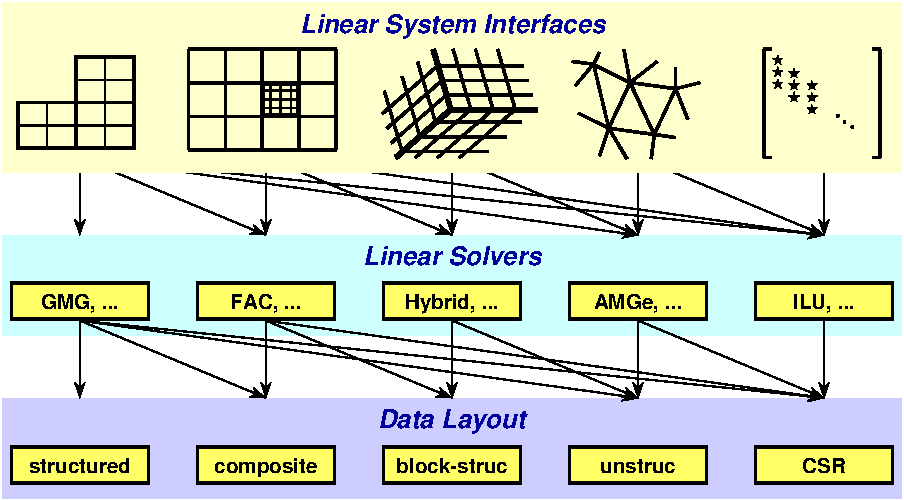
\includegraphics[width=5in]{fig_concep_iface}
\caption{%
Graphic illustrating the notion of conceptual interfaces.}
\label{fig-conceptual-interface}
\end{figure}

Generally, a user should choose the most specific interface that
matches their application, because this will allow them to use
specialized and more efficient solvers and preconditioners without
losing access to more general solvers.  For example, the second row of
Figure~\ref{fig-conceptual-interface} is a set of linear solver
algorithms.  Each linear solver group requires different information
from the user through the conceptual interfaces.  So, the geometric
multigrid algorithm (GMG) listed in the left-most box, for example,
can only be used with the left-most conceptual interface.  On the
other hand, the ILU algorithm in the right-most box may be used with
any conceptual interface.  Matrix requirements for each solver and
preconditioner are provided in Chapter \ref{ch-Solvers} and in the
\hypre{} Reference Manual.  Your desired solver strategy may influence
your choice of conceptual interface.  A typical user will select a
single Krylov method and a single preconditioner to solve their system.


The third row of Figure~\ref{fig-conceptual-interface} is a list of
data layouts or matrix/vector storage schemes.  The relationship
between linear solver and storage scheme is similar to that of the
conceptual interface and linear solver.  Note that some of the
interfaces in \hypre{} currently only support one matrix/vector
storage scheme choice.  The conceptual interface, the desired solvers
and preconditioners, and the matrix storage class must all be
compatible.


%-----------------------------------------------------------------------------

\subsection{Writing your code}

As discussed in the previous section, the following decisions should
be made before writing any code:

\begin{enumerate}
\item Choose a conceptual interface. 
\item Choose your desired solver strategy.
\item  Look up matrix requirements for each solver and preconditioner.
\item Choose a matrix storage class that is compatible with your solvers and
preconditioners and your conceptual interface.
\end{enumerate}

Once the previous decisions have been made, it is time to code your
application to call \hypre{}.  At this point, reviewing the previously
mentioned example codes provided with the \hypre{} library may prove
very helpful.  The example codes demonstrate the following general structure 
of the application calls to \hypre{}:

\begin{enumerate}

\item
{\bf Build any necessary auxiliary structures for your chosen
conceptual interface.} This includes, e.g., the grid and stencil
structures if you are using the structured-grid interface.

\item
{\bf Build the matrix, solution vector, and right-hand-side vector
through your chosen conceptual interface.}  Each conceptual interface
provides a series of calls for entering information about your problem
into \hypre{}.

\item
{\bf Build solvers and preconditioners and set solver parameters
(optional).}  Some parameters like convergence tolerance are the same
across solvers, while others are solver specific.

\item
{\bf Call the solve function for the solver.}

\item
{\bf Retrieve desired information from solver.} Depending on your
application, there may be different things you may want to do with the
solution vector.  Also, performance information such as number of
iterations is typically available, though it may differ from solver to
solver.

\end{enumerate}

The subsequent chapters of this User's Manual provide the details
needed to more fully understand the function of each conceptual
interface and each solver.  Remember that a comprehensive list of all
available functions is provided in the \hypre{} Reference Manual, and
the provided example codes may prove helpful as templates for your
specific application.

%-----------------------------------------------------------------------------

%\section{Code Design}

%In this final section of the introductory chapter, the \hypre{} object
%model is briefly discussed.

